\documentclass[12pt,a4paper,openany]{article}
\usepackage{lmodern}
\usepackage[svgnames]{xcolor} % Required to specify font color
\input{../../LaTexTemplate/templates/couleurs.tex}

\usepackage{makeidx}
\usepackage[utf8]{inputenc} 
\usepackage{marvosym}
\usepackage[T1]{fontenc}
\usepackage[francais]{babel}
\usepackage[top=1.7cm, bottom=1.7cm, left=1.7cm, right=1.7cm]{geometry}
\usepackage{verbatim}
\usepackage[urlbordercolor={1 1 1}, linkbordercolor={1 1 1}, linkcolor=vert1, urlcolor=bleu, colorlinks=true]{hyperref}
\usepackage{tikz} %Vectoriel
\usepackage{listings}
\usepackage{fancyhdr}
\usepackage{multido}
\usepackage{amssymb}
\usepackage{float}
\usepackage[francais]{minitoc}
\usepackage[final]{pdfpages} 
\usepackage{graphicx} % Required for box manipulation
\usepackage{makeidx}

\newcommand{\titre}{FactDev :\\\vspace{10px} Création de devis et facture} 
\newcommand{\titreFooter}{
\includegraphics[width=2cm]{../../../images/FACT_official.png}~~~FactDev : Création de devis et facture} 
\newcommand{\subtitle}{Compte Rendu mensuel : Mois de Février}
\newcommand{\auteur}{Équipe FACT}
\newcommand{\semestre}{~}
\newcommand{\annee}{2015}
\newcommand{\logo}{../../LaTexTemplate/templates/ups.jpg}


\newcommand{\pole}{}
\newcommand{\sigle}{~}
\makeindex
\usepackage[totoc]{idxlayout}


\input{../../LaTexTemplate/templates/listings.tex}
\input{../../LaTexTemplate/templates/article.tex}
\input{../../LaTexTemplate/templates/remarquesExempleAttentionArticle.tex}
\input{../../LaTexTemplate/templates/polices.tex}
\input{../../LaTexTemplate/templates/affichageChapitreArticle.tex}


\newcommand*{\plogo}{\fbox{$\mathcal{PL}$}} % Generic publisher logo
%----------------------------------------------------------------------------------------
%	TITLE PAGE
%----------------------------------------------------------------------------------------

\newcommand*{\rotrt}[1]{\rotatebox{90}{#1}} % Command to rotate right 90 degrees
\newcommand*{\rotlft}[1]{\rotatebox{-90}{#1}} % Command to rotate left 90 degrees

\newcommand*{\titleBC}{\begingroup % Create the command for including the title page in the document
\newlength{\drop} % Command for generating a specific amount of whitespace
\drop=0.1\textheight % Define the command as 10% of the total text height

\vspace*{-50px}
\rule{\textwidth}{0.4pt}\par % Thick horizontal line
\begin{tabular}{p{8cm}p{5cm}p{6cm}}
	\begin{minipage}{8cm}
		Équipe FACT\\
		\textit{Conception et développement d'applications}\\~\\
		\small
%		\Mobilefone~06~84~33~52~93\\
%		\Letter~\texttt{antoine.roquemaurel@gmail.com}\\
		\Mundus~\url{http://fact-team.github.io}
	\end{minipage} &
	& 

	\begin{minipage}{5cm}
		\begin{center}
			
\includegraphics[width=5cm]{logo.jpg}\\
			\tiny{Rédigé avec \LaTeX{}\\Version du \today}
		\end{center}
	\end{minipage}
\end{tabular}

\vspace{\drop} % Whitespace between the top lines and title
\centering % Center all text

\vspace{100px}
\def\CP{\textit{\Huge \titre}} % Title

\settowidth{\unitlength}{\CP} % Set the width of the curly brackets to the width of the title
{\color{LightGoldenrod}\resizebox*{\unitlength}{\baselineskip}{\rotrt{$\}$}}} \\[\baselineskip] % Print top curly bracket
\textcolor{Sienna}{\CP} \\[\baselineskip] % Print title
{\color{RosyBrown}\Large \subtitle} \\ % Tagline or further description
{\color{LightGoldenrod}\resizebox*{\unitlength}{\baselineskip}{\rotlft{$\}$}}} % Print bottom curly bracket

\vfill % Whitespace between the title and the author name


{
\normalsize \LARGE Université Toulouse III -- Paul Sabatier}\\ % Author name

\vfill % Whitespace between the author name and the publisher logo
\Large \today % Year published

\rule{\textwidth}{0.4pt}\par % Thick horizontal line

\endgroup}

%----------------------------------------------------------------------------------------
%	BLANK DOCUMENT
%----------------------------------------------------------------------------------------


\makeatother
\includeonly {
}
\begin{document}
	\thispagestyle{empty} % Removes page numbers
	\titleBC 
	\newpage
	\setcounter{tocdepth}{1}
	\setcounter{secnumdepth}{3}
	
	\tableofcontents
	\newpage
	\section{Le logiciel : FactDev}
	FactDev est un logiciel de Facture \& Devis développé par l'équipe FACT dans le cadre d'un projet de Master à l'Université Paul Sabatier composé de : 
	\begin{itemize}
		\item \textbf{F}lorent Berbie
		\item \textbf{A}ntoine de Roquemaurel
		\item \textbf{C}édric Rohaut
		\item Andriamihary Manan\textbf{T}soa Razanajatovo
	\end{itemize}

	Plus d’informations sur \Mundus~\url{http://fact-team.github.io}

	Notre enseignant tuteur est Frédéric \bsc{Migeon}.

	\begin{figure}[H]
		\centering
		
\includegraphics[width=6cm]{../FACTDev.png}
		\caption{Logo de FactDev}
	\end{figure}

	\section{Période couverte}
	Du 29 Janvier 2014 au 28 Février 2015.

	\section{Résumé des travaux de la période}
	\subsection{Sprint 0}
	Début de l'analyse et de la conception du projet
	Mise en place de l'architecture pour pouvoir débuter les « \textit{Sprints} » suivants. 
	Choix des technologies (C++ avec Qt, QTest, Git, Génération de \LaTeX{}), choix de la base de données (SQLite)
	Définition des différentes « \textit{User Stories} »

	\subsection{Planning poker}
	Une fois le \textit{sprint} 0 terminé, nous avons pu mettre en place la méthode Scrum. L’une des premières choses fut de faire un « Planning Poker » afin
	de : 
	\begin{itemize}
		\item Définir un poids pour l'intégralité des \textit{Users Stories}
		\item Définir la priorité pour l'intégralité des \textit{Users Stories}
		\item Répartir les \textit{Users Stories} en différents \textit{sprints} et \textit{releases}. 
	\end{itemize}

	\subsection{Sprint 1}
	L'ensemble des << \textit{issues} >> ou « \textit{User Stories} » sont définis dans GitHub et un document « \textit{BackLog} » (Google Sheets). Dès qu'un membre de l'équipe
	souhaite développer une nouvelle fonctionnalité, il se l'assigne. Lors du premier \textit{Sprint}, nous avons développé l'interface générale de
	l'application et créer la base de données et les interactions principales entre nos objets et celle-ci. Nous avons également programmé l'ajout des
	informations de l'utilisateur et la création d’un nouveau client, sa modification ou suppression. Une barre de recherche fonctionnelle a également
	été implémenté, ainsi que des filtres (recherche sur les clients ou les sociétés). Enfin, nous avons mis en place des tests unitaires pour assurer
	le bon fonctionnement de parties du code. 
	Ce \textit{sprint}, ainsi que ceux qui suivent, fournissent un manuel d’utilisateur à jour des fonctionnalités venant d’être implémentées.  
	\textit{Sprint} 2 en cours (première semaine du \textit{sprint})

	Durant la première semaine du second \textit{Sprint}, nous avons ajouté la possibilité de créer de nouveaux projets et de les associer à un client. Il est
	également possible de modifier ou supprimer un projet. L'interface générale de l’application a également été modifié pour répondre aux nouvelles
	fonctions ajoutées. Lors de l'ajout d’un nouvel élément (projet, client, …), certains champs doivent obligatoirement être renseignés avec une
	syntaxe correcte pour que cela puisse être sauvegardé. 

	\section{Travaux effectivement réalisés en fin de période}
	L'ensemble des « \textit{User} » et « \textit{Technical Stories} » ont été réalisé dans les temps. La réalisation de celles-ci signifie que les considère comme
	finis, c'est-à-dire que la fonction fait bien ce qu'on lui demande, que le code est facile à lire, peu complexe et correctement documenté. 
	En plus de ce que nous avions initialement prévu, nous avons également réalisé un site internet présentant l'équipe de développement, le projet et
	divers liens propres à ce projet :
	\begin{itemize}
		\item Manuel d’utilisateur : \Mundus~\url{http://fact-team.github.io/doc/usermanual.pdf}
		\item Code source et ressources GitHub : \Mundus~\url{https://github.com/FACT-Team/FactDev}
		\item Documentation :
			\begin{itemize}
				\item Au format HTML : \Mundus~\url{http://fact-team.github.io/doc/html/index.html}
				\item Au format PDF :  \Mundus~\url{http://fact-team.github.io/doc/latex/refman.pdf}
			\end{itemize}
	\end{itemize}

	\section{Charge de travail pour le groupe}
	\subsection{Charge estimé}
	\begin{table}[H]
		\centering
		\begin{tabular}{l|c|c}
			\textbf{Désignation} & \textbf{Fréquence} & \textbf{Total}\\
			\hline
			Réunions tuteur & 1h / semaine & 4h\\
			Réunions de travail & 2.5h / semaine & 10h\\
			Travail personnel & 8h / semaine & 24h
		\end{tabular}
		\caption{Charge de travail constatée}
	\end{table}

	\subsection{Charge constatés}
	\begin{table}[H]
		\centering
		\begin{tabular}{l|c|c}
			\textbf{Désignation} & \textbf{Fréquence} & \textbf{Total}\\
			\hline
			Réunions tuteur & 1h / semaine & 4h\\
			Réunions de travail & \textbf{4h / semaine} & \textbf{16h}\\
			Travail personnel & 8h / semaine & 24h
		\end{tabular}
		\caption{Charge de travail estimée}
	\end{table}
	Nous avions prévu deux heures et demi de réunions de travail avec tout le groupe. Cependant, au début du projet, trois membres du groupes
	connaissaient peu les technologies choisies. Il fut donc préférable de travailler dans la même pièce à la manière d’un « \textit{open space} ». 
	
	Si un des développeurs avait un problème qu'il ne parvenait pas à résoudre, les autres développeurs lui venaient en aide. Ceci contribue à la cohésion
	d'équipe, à la réalisation d’un projet homogène et un avancement plus rapide du projet. 
	
	Cette démarche a aussi été faite dans le but de faire
	progresser rapidement les développeurs afin que ces derniers, ne connaissant pas la technologie, ne bloquent pas sur des problèmes qui sont, pour
	la plupart, mineurs.

	\section{Problèmes techniques constatés}
	\begin{itemize}
		\item Installation de l'outils Sonar
		\item Choix de l'outil tests : QTest a été adopté plutôt que GTest qui posait des problèmes de compatibilité entre les systèmes 
		\item Problèmes de compatibilités entre systèmes : Mac / Windows
		\item Formation sur les technologies
	\end{itemize}
	\section{Décisions prises}
	Avant de rentrer dans le vif du sujet, l'équipe a tenu à mettre en place des standards afin d’assurer une meilleure gestion du projet, une
	meilleure cohésion d’équipe et un code plus homogène. 
	\subsection{La méthode \textit{Scrum}}
	Pour une bonne utilisation de cette méthode, nous avons choisis : 
	\begin{itemize}
		\item Le nombre de versions livrables (\textit{Releases}) et le nombre de \textit{Sprints} par \textit{Release}. Dans notre cas nous avons
			deux \textit{releases} contenant chacune trois \textit{sprints}
		\item Les \textit{User/Technical stories} pour chaque \textit{sprint}
		\item De faire réunions quotidiennes (mêlées)
	\end{itemize}

	\subsection{Utilisation de Github}
	Nous avons rédigés un wiki sur notre compte Github, comprenant :
	\begin{itemize}
		\item Les conventions d’écritures (normalisation des noms de variables, de méthodes, de l'indentation, \ldots)\newline
			\Mundus~\url{https://github.com/FACT-Team/Team-Organization/wiki/Conventions-de-codage-en-C--}
		\item un tutoriel sur Git\newline
			\Mundus~\url{https://github.com/FACT-Team/Team-Organization/wiki/Mini-Tuto-Git}
		\item Un cours explicatif sur notre façon de développer sous Git : une user story aura une nouvelle branche \newline
			\Mundus~\url{https://github.com/FACT-Team/FactDev/wiki/Workflow}
	\end{itemize}

	\begin{figure}[H]
		\centering
		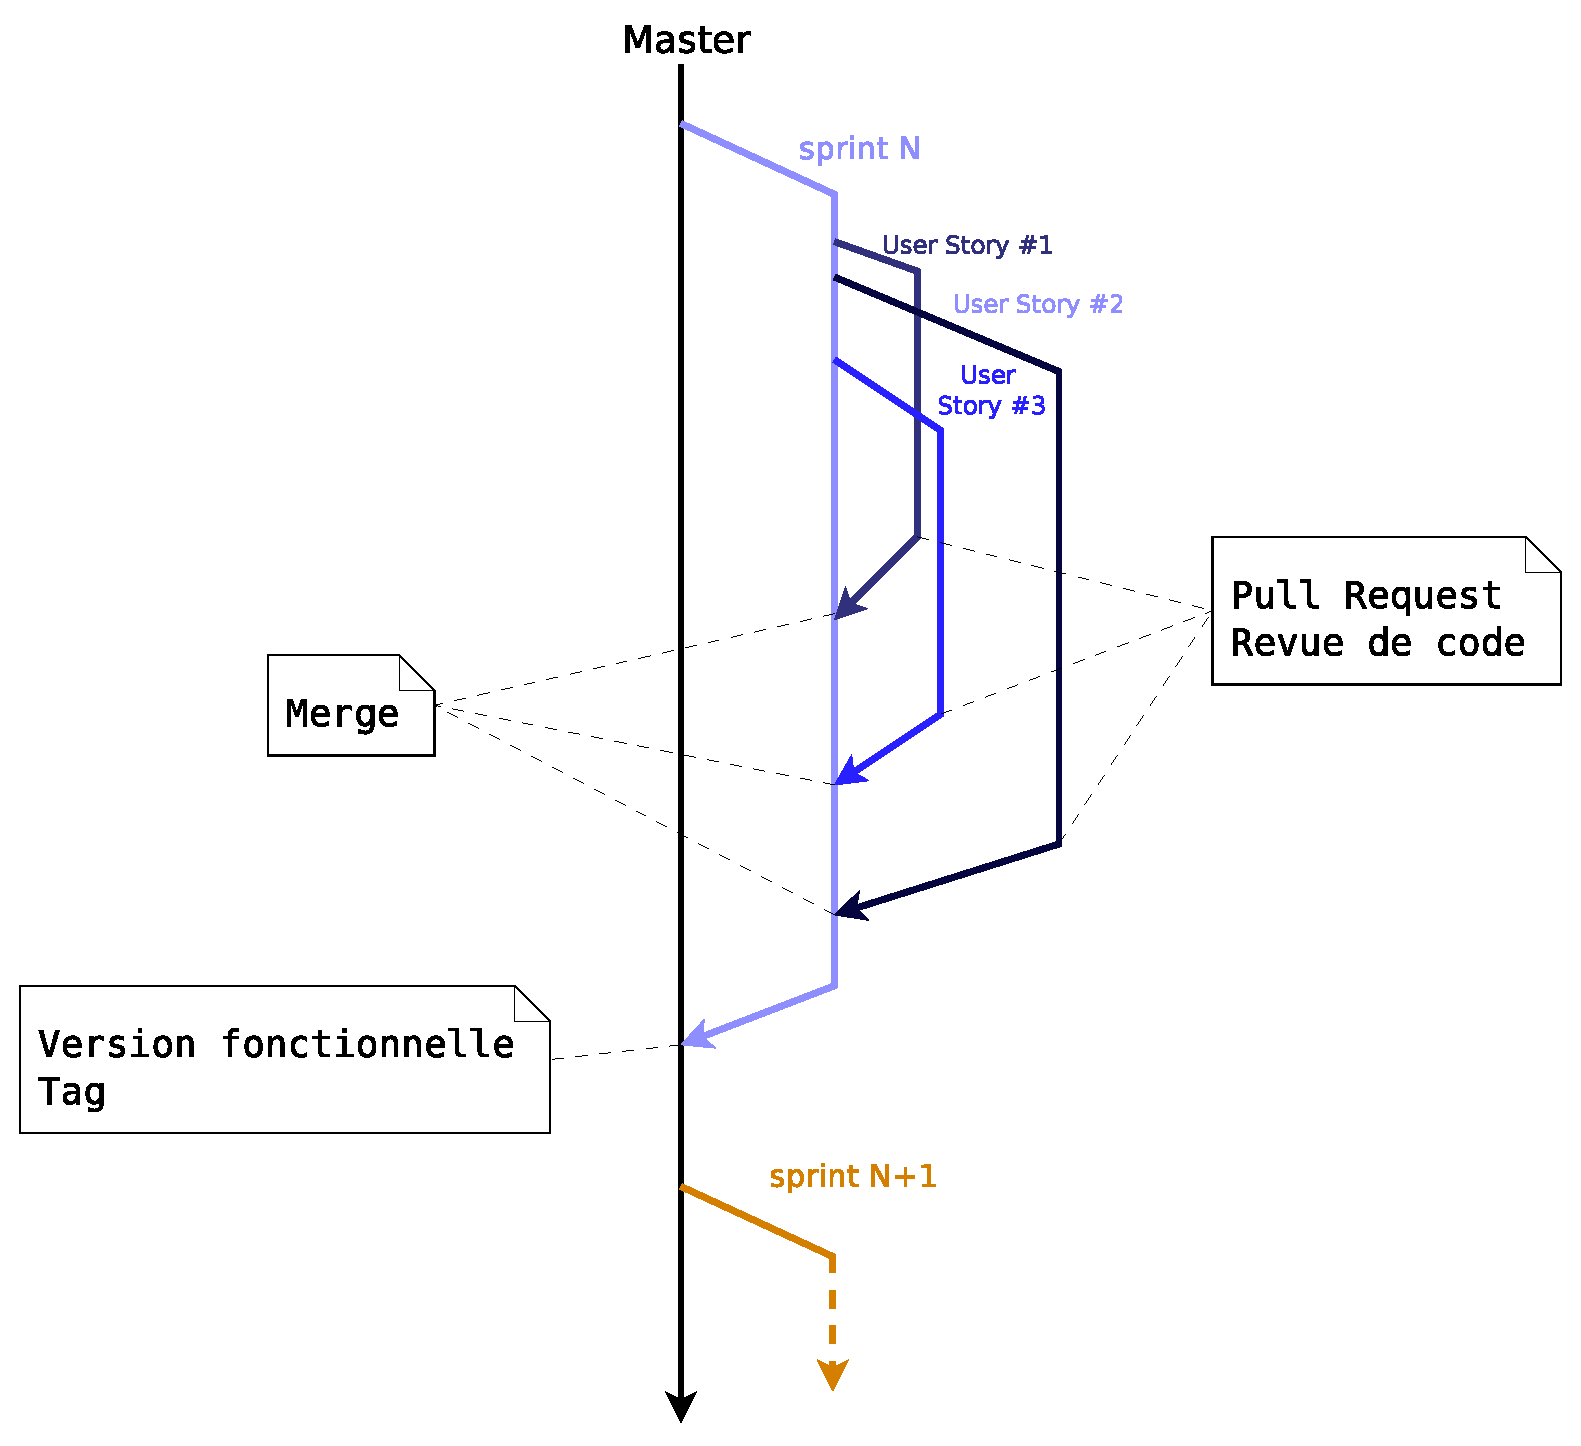
\includegraphics[width=11cm]{BranchingWorkflow.eps}
		\caption{Principe du « \textit{Git Branching Workflow} »}
	\end{figure}
	\subsection{Assurer une revue de code}
	    Le développeur ayant programmé une nouvelle fonctionnalité (et donc créé une nouvelle branche au projet sur Git) mentionne via une <<
		\textit{Pull Request} >> qu'il a terminé.  Les autres membres de l'équipe en sont informés. 
		
		Un de ses membres se charge de la revue de code, ce qui signifie
		qu'il devait vérifier que cela fonctionne et que le code est propre, facilement lisible, peu complexe et commenté. Une fois que tous ces
		éléments ont été revus et jugés valides, la branche est fusionnée à la branche principale (nommée Master) du projet. 

\end{document}
